\documentclass{beamer}

\usepackage[utf8]{inputenc}
\usecolortheme{beaver}
\usepackage{caption}
\usepackage{subcaption}
\usepackage{mathtools}
\usepackage{todonotes}
\usepackage{bm}
\usepackage{listings}

\def\ci{\perp\!\!\!\!\!\perp}

\newtheorem{proposition}{Proposition}

\begin{document}

\title{A Simple Unified Approach to Testing High-Dimensional Conditional Independencies}
\author {Ankur Ankan \and Johannes Textor}
\institute{Radboud University}
\date{}
\maketitle

\begin{frame}
	\frametitle{Overview}
	\tableofcontents
\end{frame}

\section{Motivation}
\begin{frame}
	\frametitle{Motivation: Example DAG / Causal Bayesian Network}
	\begin{figure}
		\centering
		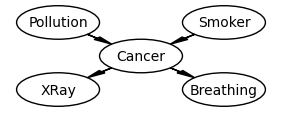
\includegraphics[scale=0.6]{imgs/example_dag.png}
		\caption*{An example of Directed Acyclic Graph (DAG) \footnotemark}
	\end{figure}
	\begin{itemize}
		\setlength\itemsep{1em}
		\item Random variables are represented using nodes.
		\item Directed edges represent direct causal link between variables.
		\item Each variable is conditionally independent of all non-descendants given its parents. E.g. \newline
			\hspace*{20pt} $ \text{\emph{XRay}} \ci \text{\emph{Pollution}} | \text{\emph{Cancer}} $ \newline
			\hspace*{20pt} $ \text{\emph{Breathing}} \ci \text{\emph{Smoker}} | \text{\emph{Cancer}} $
	\end{itemize}
	\footnotetext[1]{\footnotesize{K. B. Korb, A. E. Nicholson. Bayesian Artificial Intelligence}}
\end{frame}

\begin{frame}[fragile]
	\frametitle{Motivation: Model Testing}
	\begin{itemize}
		\setlength\itemsep{1em}
		\item In applied research, most of the DAGs are made by hand
			based on domain knowledge.
		\item Important to test whether the model is consistent with the data.
		\item Conditional Independence (CI) tests can be used to verify model structure.
	\end{itemize}
	\vspace{1em}
	\begin{figure}
 	\begin{verbatim}
                              x2 df    p.value
 Brth _||_ Pllt | Cncr 4.7571803  2 0.09268115
 Brth _||_ Smkr | Cncr 9.0058063  2 0.01107679
 Brth _||_ XRay | Cncr 1.9104270  2 0.38472999
 	\end{verbatim}
		\caption*{Example model testing output from R package \emph{dagitty}}
	\end{figure}

\end{frame}

\begin{frame}
	\frametitle{Motivation: Structure Learning}
	\begin{itemize}
		\setlength\itemsep{1em}
		\item CI implies that no direct causal link exists between the variables. \newline
			$ \text{\emph{XRay}} \ci \text{\emph{Smoker}} | \text{\emph{Cancer}} \implies \text{No edge b/w \emph{XRay} and \emph{Smoker}} $

		\item Constraint-Based structure learning algorithms like PC
			and FCI use CI tests to systematically search for CIs
			in the dataset to determine model skeletons.
	\end{itemize}
	\begin{figure}
		\centering
		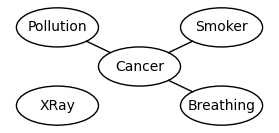
\includegraphics[scale=0.6]{imgs/example_sl.png}
		\caption*{Structure Learning Example}
	\end{figure}
\end{frame}

\section{Background}
\begin{frame}
	\frametitle{(Conditional) Independence}
	\begin{block}{Independence}
		Two random variables $ X $ and $ Y $ are independent,
		$ X \ci Y $ if and only if $ P(X, Y) = P(X) \cdot P(Y) $.
	\end{block}
	\vspace{1em}

	\begin{block}{Conditional Independence}
		Two random variables $ X $ and $ Y $ and are said to be
		conditionally independent given $ \bm{Z} $, $ X \ci Y | \bm{Z}
		$ if and only if for all $ z $ with $ p(z) > 0 $, $ P(X, Y |
		Z=z) = P(X | Z=z) \cdot P(Y | Z=z) $
	\end{block}
\end{frame}

\begin{frame}
	\frametitle{CI Testing is Difficult}
	\begin{figure}
		\centering
		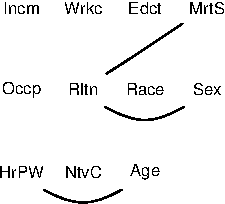
\includegraphics[scale=0.7]{imgs/sl-adult-mi-crop.pdf}
		\caption*{Learned structure for US census income dataset using chi-square test}
	\end{figure}
	\begin{itemize}
		\item Testing for CI is much harder compared to testing for
			non-conditional independence.
		\item Especially in case of high cardinality or high number of
			conditional variables.
		\item In the continuous case, no test can exist which is calibrated and
			has power over all distributions where CI is True. \footnotemark
		\item Many different approaches and tests have been proposed.
	\end{itemize}

	\footnotetext[2]{\footnotesize{Shah, Rajen D., and Jonas Peters. "The hardness of conditional independence testing and the generalised covariance measure." The Annals of Statistics, 2020}}
\end{frame}

\begin{frame}
	\frametitle{Main classes of tests}
	\begin{itemize}
		\setlength\itemsep{1em}
		\item Stratification based tests
		\item Variable Importance based tests
		\item Residulaization based tests
	\end{itemize}
\end{frame}

\begin{frame}
	\frametitle{Stratification Based Tests}
	\begin{itemize}
		\setlength\itemsep{1em}
		\item Most common type for discrete variables. E.g. chi-square,
			mutual information based test etc. 
		\item Converts CI test into simple independence test by splitting 
			the dataset.
		$ D[X, Y, \bm{Z}] = \{ D[X, Y, \bm{Z}=\bm{z_1}], D[X, Y, \bm{Z}=\bm{z_2}], \cdots \} $	
		\item Runs test on each stratum and then combines the results.
		\item As the number of conditional variables is increased, exponentially
			less data is available in each stratum.
		\item Looses power when number of conditonal variables
			are increased.
	\end{itemize}
\end{frame}

\begin{frame}
	\frametitle{Variable Importance Tests}
	\begin{itemize}
		\setlength\itemsep{1em}
		\item Based on comparing the probability models: $\hat{p}(x |
			y, z) $ and $ \hat{p}(x | z) $. E.g. Stochastic
			Complexity-Based Conditional Independence Test (SCCI) \footnotemark.
		\item If the simpler model doesn't fit significantly worse, implies $ X \ci Y | Z $.
		\item Can utilize any statistical model for which a reasonable goodness
			of fit exist.
		\item Inherently asymmetrical. The result of $ X \ci Y | Z $
			can be different from $ Y \ci X | Z $.
	\end{itemize}
	\footnotetext[3]{\footnotesize Marx, Alexander, and Jilles Vreeken. "Testing conditional independence on discrete data using stochastic complexity." PMLR, 2019}

\end{frame}

\begin{frame}
	\frametitle{Residualization Based Tests}
	\begin{itemize}
		\setlength\itemsep{1em}
		\item Uses two estimators $ \mathbb{E}[X| Z] $ and $
			\mathbb{E}[Y | Z] $ and checks for the multiplicative
			association between the residuals. E.g.
			Partial Correlation test, generalized covariance measure etc.
		\item Relies on the theorem from Daudin [1980] \footnotemark 
			that under CI, if the estimators have ``valid'' residuals
			such that $ \mathbb{E}[R_{X|Z}] = \mathbb{E}[R_{Y|Z}] = 0 $,
			then $ \mathbb{E}[R_{X|Z} R_{Y|Z}] = 0 $.
		\item Any estimator can be used as long as it has ``valid'' residuals.
		\item No residualization based test exists for categorical or ordinal variables.
	\end{itemize}
	\footnotetext[4]{\footnotesize Daudin, J. J. "Partial association measures and an application to qualitative regression." Biometrika, 1980}
\end{frame}

\section{Proposed Method}
\begin{frame}
	\frametitle{Proposed Method}
	\begin{itemize}
		\setlength\itemsep{1em}
		\item Residualization based approach.
		\item Uses Li-Shepherd (LS) residuals \footnotemark.
		\item Any unbiased estimator can be used. We show empirical results using Logistic Regression (GLM) and Random Forest (RFT).
	\end{itemize}
	\footnotetext[5]{\footnotesize C. Li and B. E. Shepherd. "A new residual for ordinal outcomes." Biometrika, 2012}
\end{frame}

\begin{frame}
	\frametitle{LS-Residuals}
	Given an ordinal variable $ Y $ and an estimate $ \hat{p}(y) $ of $
	p(y) $, LS-Residual for sample $ y_i $ is defined as:
	$$ R_{y_i} = \hat{p}(Y < y_i) - \hat{p}(Y > y_i) $$
	\vspace{1em}

	For the binary case with $ Y \in \{0, 1\} $:
	$$ R_{y_i} = y_i - \hat{p}(Y = 1) $$
	\vspace{1em}

	For the conditional case for sample $ (y|z)_i $,
	$$ R_{y_i | z_i} = \hat{p}(Y < y_i | Z=z_i) - \hat{p}(Y>y_i|Z=z_i) $$

\end{frame}

\begin{frame}
	\frametitle{Proposition}
	If $ X \ci Y | Z $ and $ \hat{p}(x|z) $ and $ \hat{p}(y|z) $ are asymptotically
	unbiased estimators of $ p(x|z) $ and $ p(y|z) $ respectively, then 
	$ \mathrm{Cov}(R_{\bm{x}|\bm{z}}, R_{\bm{y}|\bm{z}}) = 0 $ in large sample limit.	
	\vspace{1em}

	\begin{itemize}
		\setlength\itemsep{1em}
		\item For asymptotically unbaised estimators, LS-Residuals
			gives ``valid''residuals: $ E[R_{X|Z}] = E[R_{Y|Z}] = 0
			$.
		\item Under $ X \ci Y | \bm{Z} $, valid
			residuals imply $ \mathbb{E}[R_{X|Z} R_{Y|Z}] = 0 $ \footnotemark.
	\end{itemize}
	\footnotetext[6]{\footnotesize Daudin, J. J. "Partial association measures and an application to qualitative regression." Biometrika, 1980}
\end{frame}

\begin{frame}
	\frametitle{Test Statistic: Both ordinal variables}
	$$ Q_1(\bm{x}, \bm{y}) = \frac{1}{n} \frac{(R_{\bm{x}} \cdot R_{\bm{y}})^2}{\bm{var}(R_{\bm{x}} R_{\bm{y}})} $$

	If $ X \ci Y | Z $, then asymptotically $ Q_1(\bm{x}, \bm{y}) \sim \chi^2(1) $.

	\vspace{1em}
	\begin{itemize}
		\setlength\itemsep{1em}
		\item Train two estimators: $ E_X = \mathbf{x} \sim \mathbf{z} $ and $ E_Y = \mathbf{y} \sim \mathbf{z} $
		\item Make probability predictions for each data point: $ \hat{p}(x|z) $ and $ \hat{p}(y|z) $ using $ E_X $ and $ E_Y $ respectively.
		\item Compute the LS-Residuals for each data point: $ R_{\mathbf{x}} $ and $ R_{\mathbf{y}} $.
		\item Use $ R_{\mathbf{x}} $ and $ R_{\mathbf{y}} $ to compute $ Q_1 $.
	\end{itemize}

\end{frame}

\begin{frame}
	\frametitle{Test Statistic: Both ordinal variables}
	$$ Q_1(\bm{x}, \bm{y}) = \frac{1}{n} \frac{(R_{\bm{x}} \cdot R_{\bm{y}})^2}{\bm{var}(R_{\bm{x}} R_{\bm{y}})} $$

	If $ X \ci Y | Z $, then asymptotically $ Q_1(\bm{x}, \bm{y}) \sim \chi^2(1) $.

	\vspace{1em}
	\begin{itemize}
		\setlength\itemsep{1em}
		\item From the first proposition, population mean $ \mathbb{E}[R_X R_Y] = 0 $
		\item From Central Limit Theorem, the standardized sample mean of $ R_x R_y $, $ \frac{1}{n} \frac{R_x \cdot R_y}{\sigma(R_xR_y)} \sim \mathcal{N}(0, \frac{1}{\sqrt{n}}) $.
		\item $ Q_1 $ is chi-squared distributed with $ 1 $ degree of freedom (df).
	\end{itemize}
\end{frame}

\begin{frame}
	\frametitle{Test Statistic: One ordinal and one categorical}
	$$ Q_2(\bm{x}, \bm{y}) = \frac{1}{n} (d \times \hat{\Sigma}_d^{-1} \times d^T) $$
	where $ d = (R_{\mathbb{I}(\mathbf{x}=1)} \cdot R_{\mathbf{y}}, \, \ldots \ ,
		R_{\mathbb{I}(\mathbf{x}=k-1)} \cdot R_{\mathbf{y}})$ and $ \hat{\Sigma}_d $ is the covariance matrix.

	\vspace{1em}
	If $ X \ci Y | Z $, then asymptotically $ Q_2(\bm{x}, \bm{y}) \sim \chi^2(k-1) $.

	\begin{itemize}
		\setlength\itemsep{1em}
		\item Dummy/one-hot encode the categorical variable.
		\item Similar to last case, train two estimators: $ E_X = \mathbf{x} \sim \mathbf{z} $ and $ E_Y = \mathbf{y} \sim \mathbf{z} $ and make probability predictions using them: $ \hat{p}(x|z) $ and $ \hat{p}(y | z) $.
		\item Compute the LS residuals for each dummy variable assuming them to be binary ($ R_{\mathbf{x}} $) and the ordinal variable ($ R_{\mathbf{y}} $).
		\item $ d $ is the product of residual from each dummy variable and the ordinal variable's residual.

	\end{itemize}
\end{frame}

\begin{frame}
	\frametitle{Test Statistic: One ordinal and one categorical}
	$$ Q_2(\bm{x}, \bm{y}) = \frac{1}{n} (d \times \hat{\Sigma}_d^{-1} \times d^T) $$
	where $ d = (R_{\mathbb{I}(\mathbf{x}=1)} \cdot R_{\mathbf{y}}, \, \ldots \ ,
		R_{\mathbb{I}(\mathbf{x}=k-1)} \cdot R_{\mathbf{y}})$ and $ \hat{\Sigma}_d $ is the covariance matrix.

	\vspace{1em}
	If $ X \ci Y | Z $, then asymptotically $ Q_2(\bm{x}, \bm{y}) \sim \chi^2(k-1) $.

	\begin{itemize}
		\item Under CI, each component of $ d $ is asymptotically normal.
		\item Components of $ d $ are linearly correlated. Hence, $ d $ is 
			a multivariate gaussian distributed.
		\item $ Q_2 $ is chi-squared distributed with $ k-1 $ df.
	\end{itemize}
\end{frame}

\begin{frame}
	\frametitle{Test Statistic: Both categorical}

	$$ Q_3(\bm{x}, \bm{y}) = \frac{1}{n} (d \times \hat{\Sigma}_d^{-1} \times d^T) $$

	where 
	\begin{eqnarray*}
		d &  =  & (R_{\mathbb{I}(\mathbf{x}=1)} \cdot R_{\mathbb{I}(\mathbf{y}=1)}, \, \ldots \ ,
		R_{\mathbb{I}(\mathbf{x}=k-1)} R_{\mathbb{I}(\mathbf{y}=1)}, \, \ldots \, ,
		\\
	 	& & R_{\mathbb{I}(\mathbf{x}=1)} \cdot R_{\mathbb{I}(\mathbf{y}=r-1)}, \, \ldots \ ,
		R_{\mathbb{I}(\mathbf{x}=k-1)} R_{\mathbb{I}(\mathbf{y}=r-1)}
		)
	\end{eqnarray*}
	\vspace{1em}

	If $ X \ci Y | Z $, then asymptotically $ Q_3(\bm{x}, \bm{y}) \sim \chi^2((k-1)(r-1)) $.

	\begin{itemize}
		\setlength\itemsep{1em}
		\item Same as the last case, $ Q_3(\bm{x}, \bm{y}) $ is chi-squared distributed 
			with $ (k-1)(r-1) $ df.
	\end{itemize}
\end{frame}

\begin{frame}
	\frametitle{Test Summary}
	\begin{enumerate}
		\setlength\itemsep{1em}
		\item If $\mathbf{Z} = \emptyset $ , do a non-conditional chi-squared test.
		\item If either $ X $ or $ Y $ are non-binary categorical,
			dummy/one-hot encode them.
		\item Train two estimators $ E_x = \bm{x} \sim \bm{z} $ and
			$ E_y = \bm{y} \sim \bm{z} $
		\item Make probability predictions using these two estimators 
			$ \hat{p}(x) = E_x(\bm{z}) $ and $ \hat{p}(y) =
			E_y(\bm{\bm{z}}) $.
		\item Use predictions and true values to compute LS-Residuals $ R_{\bm{x}|\bm{z}} $ and $ R_{\bm{y}|\bm{z}} $.	
		\item Compute the test statistic and df.
	\end{enumerate}
\end{frame}

\section{Empirical Results}

\begin{frame}
	\frametitle{Empirical Analysis: Calibration}
	\begin{figure}
		\centering
		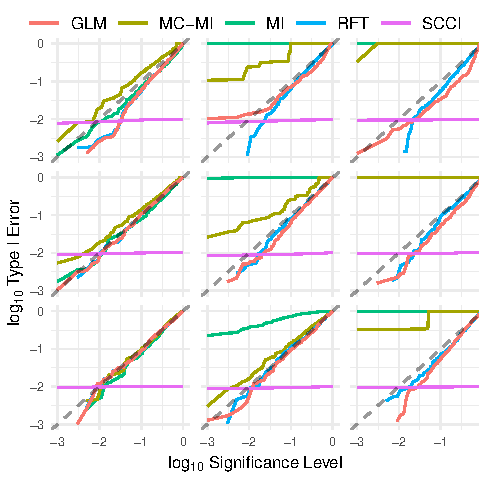
\includegraphics[scale=0.8]{imgs/calibration_add_vars.pdf}
		\caption*{Type I error vs significance level for sample sizes (top to
		bottom): $ [20, 40, 80] $ and number of conditional variables (left to
		right): $ [1, 3, 5] $ on conditionally independent simulated binary
		datasets.}
	\end{figure}
\end{frame}

\begin{frame}
	\frametitle{Empirical Analysis: Discrimination}
	\begin{figure}
		\centering
		\begin{subfigure}{0.8 \textwidth}
			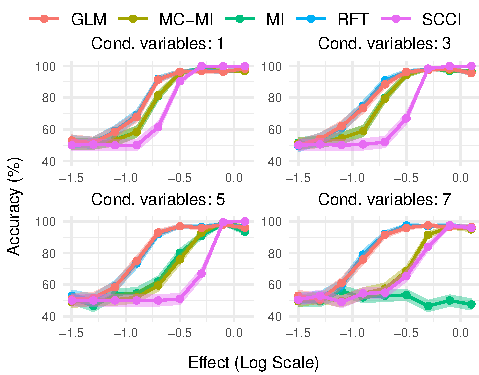
\includegraphics{imgs/accuracy.pdf}
		\end{subfigure}%
		\begin{subfigure}{0.2 \textwidth}
			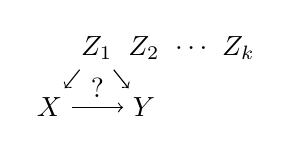
\begin{tikzpicture}[yscale=.75, xscale=.6]
				\node (x) at (0,0) {$X$};
				\node (y) at (2,0) {$Y$};
				\node (z) at (1,1) {$Z_1$};
				\node at (2,1) {$Z_2$};
				\node at (3,1) {$\ldots$};
				\node at (4,1) {$Z_k$};
				\draw [->] (x) edge node [midway, above] {?} (y);
				\draw [->] (z) -- (y);
				\draw [->] (z) -- (x);
			\end{tikzpicture}
		\end{subfigure}
		\caption*{(a) Accuracy (shading: mean $\pm$ standard error, $N=200$)
		of classifying simulated binary datasets (sample size: $1000$)
		as conditionally dependent or independent. (b) The data generating DAG.}
	\end{figure}

\end{frame}

\begin{frame}
	\frametitle{Empirical Analysis: Discrimination (Ordinal)}
	\begin{figure}
		\centering
		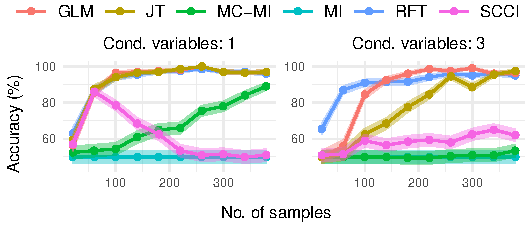
\includegraphics{imgs/accuracy_ordinal.pdf}
		\caption*{Accuracy (shading: mean $\pm$ standard error) of
		classifying simulated ordinal data (8 levels per variable) as
		conditionally dependent or independent.}	
	\end{figure}
	\footnotetext[7]{JT = Jonckheere-Terpstra test}
\end{frame}

\begin{frame}
	\frametitle{Applications: Model testing}
	\begin{figure}
		\centering
		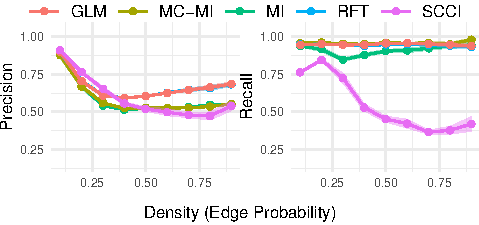
\includegraphics{imgs/model_testing.pdf}
		\caption*{Precision and recall (shading: mean $\pm$ standard
		error) of testing implied CIs and equal number of randomly
		generated CIs in binary datasets (sample size: $1000$)
		simulated from random DAGs on $ 20 $ variables.}
	\end{figure}
\end{frame}

\begin{frame}
	\frametitle{Applications: Structure Learning}
	\begin{figure}
		\centering
		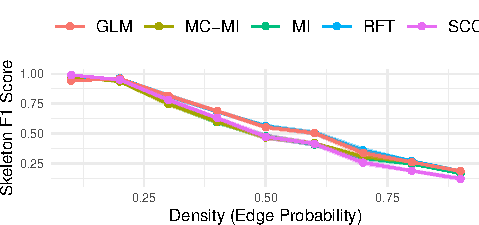
\includegraphics{imgs/sl_density.pdf}
		\caption*{Structure learning on simulated data. F1-score
		(shading: mean $\pm$ standard error) of the learned model
		skeletons for randomly generated DAGs with $20$ variables and
		varying edge probabilities.}
	\end{figure}
\end{frame}

\begin{frame}
	\frametitle{Applications: Structure Learning}
	\begin{figure}
		\centering
		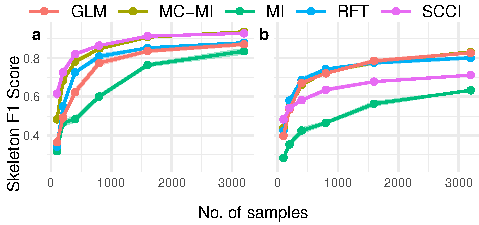
\includegraphics{imgs/sl.pdf}
		\caption*{Structure learning on (a) ``alarm'', and (b)
		``insurance'' datasets.  F1-score (shading: mean $\pm$ standard
		error, $N=10$) of the learned model skeletons.}
	\end{figure}
\end{frame}

\begin{frame}
	\frametitle{Applications: Structure Learning}
	\begin{figure}
		\centering
		\begin{subfigure}{0.5\textwidth}
			\centering
			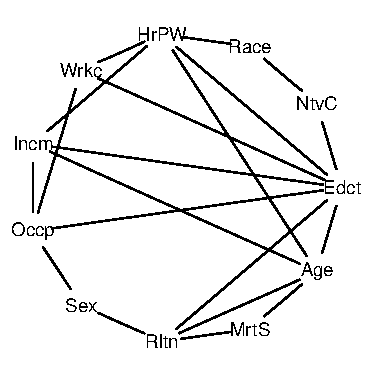
\includegraphics[scale=0.85]{imgs/sl-adult-rf.pdf}
			\caption*{}
			\label{fig:sl_adult_model}
		\end{subfigure}%
		\begin{subfigure}{0.5\textwidth}
			\centering
			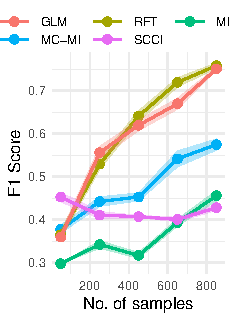
\includegraphics{imgs/adult_F1.pdf}
			\caption*{}
			\label{fig:sl_adult}
		\end{subfigure}
		\caption*{Structure learning on US census income dataset. (a)
		Learnt skeleton using RFT. (b) F1-score (shading: mean $\pm$
		standard error, $N=10$) when comparing $d$-connected variable
		pairs from the CPDAG to correlated variable pairs in the
		dataset.}
	\end{figure}
\end{frame}

\begin{frame}
	\frametitle{Runtime Analysis}
	\begin{figure}
		\centering
		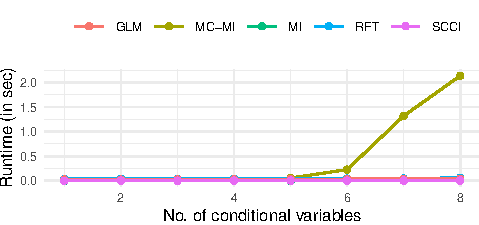
\includegraphics{imgs/runtime.pdf}
		\caption*{Runtime (shading: mean $\pm$ standard error, $N=100$)
		for CI tests with varying numbers of conditional variables and
		$1000$ samples per dataset.
		}
	\end{figure}
\end{frame}

\section{Conclusion}
\begin{frame}
	\frametitle{Conclusion/Future Work}
	\begin{itemize}
		\setlength\itemsep{1em}
		\item A residualization based CI test for categorical and
			ordinal variables.
		\item Properties: 1) Simple to implement; 2) Interpretable chi-square test statistic; 3) Symmetric by construction; 4) Computationally feasible
		\item Performs reasonably well for low number of
			conditional variable but performs better for high
			number of conditional variables.
		\item For structure learning, a hybrid approach can be used with other
			tests.
		\item Since Random Forests can work with combination of discrete and 
			continuous variables, can possibly be extended to a single 
			unified test.
	\end{itemize}
\end{frame}

\begin{frame}
	\begin{center}
		\Huge{Questions / Suggestions}
	\end{center}
\end{frame}

\end{document}
